%%%%%%%%%%%%%%%%%%%%%%%%%%%%%%%%%%%%%%%%%%%%%%%%%%%%%%%%%%%%%%%%%%%%%%%%%%%%%%%%%%%%%%%%%%%%%%%%%%%%%
% This template is distributed with ABSOLUTELY NO WARRANTY.
% It serves as a guideline and constitutes a basic structure for a
% thesis/dissertation. The user assumes full responsibility for formatting
% and typesetting their document and for verifying that all the thesis
% requirements set by the University of Tennessee are met. Please refer to the most
% recent UT thesis guide (http://gradschool.utk.edu/thesesdissertations/formatting/)
% or contact the thesis consultant (http://gradschool.utk.edu/thesesdissertations/).
% Please report any bugs to the thesis consultant.
%%%%%%%%%%%%%%%%%%%%%%%%%%%%%%%%%%%%%%%%%%%%%%%%%%%%%%%%%%%%%%%%%%%%%%%%%%%%%%%%%%%%%%%%%%%%%%%%%%%%%
% O P T I O N S:
% 1. thesis/dissertation
% 2. monochrome
% 3. all options provided by the report class
%%%%%%%%%%%%%%%%%%%%%%%%%%%%%%%%%%%%%%%%%%%%%%%%%%%%%%%%%%%%%%%%%%%%%%%%%%%%%%%%%%%%%%%%%%%%%%%%%%%%%
%First, is this a thesis or dissertation? Choose one by commenting out the one you don't need:
%\documentclass[thesis,letterpaper,12pt]{utthesis} % thesis
\documentclass[thesis,letterpaper,12pt]{utthesis} %dissertation
% some alternatives are:
%\documentclass[thesis,monochrome,letterpaper,12pt]{utthesis} %thesis, monochrome text
\renewcommand{\baselinestretch}{1.5} 	 % line Spacing
%%%%%%%%%%%%%%%%%%%%%%%%%%%%%%%%%%%%%%%%%%%%%%%%%%%%%%%%%%%%%%%%%%%%%%%%%%%%%%%%%%%%%%%%%%%%%%%%%%%%%
% TO DO: FILL IN YOUR INFORMATION BELOW - READ THIS SECTION CAREFULLY
%%%%%%%%%%%%%%%%%%%%%%%%%%%%%%%%%%%%%%%%%%%%%%%%%%%%%%%%%%%%%%%%%%%%%%%%%%%%%%%%%%%%%%%%%%%%%%%%%%%%%
\title{Semi-Empirical Modeling and Implementation of Hybrid K-Edge Densitometry for Pyroprocessing Applications}	       	% title of thesis/dissertation
\author{Michael P. Cooper}                			% author's name
\copyrightYear{2018}            				% copyright year of your thesis/dissertation
\graduationMonth{May}           				% month of graduation for your thesis/dissertation
\degree{Master of Science}	    			% degree: Doctor of Philosophy, Master of Science, Master of Engineering...
\university{The University  of Tennessee, Knoxville}	% school name
%%%%%%%%%%%%%%%%%%%%%%%%%%%%%%%%%%%%%%%%%%%%%%%%%%%%%%%%%%%%%%%%%%%%%%%%%%%%%%%%%%%%%%%%%%%%%%%%%%%%%
% LOAD SOME USEFUL PACKAGES. 
% No need to change anything here, although if you'd like to add packages you can do that here. Note that packages preloaded with the utthesis class are: amsmath,amsthm,amssymb,setspace,geometry,hyperref,and color
%%%%%%%%%%%%%%%%%%%%%%%%%%%%%%%%%%%%%%%%%%%%%%%%%%%%%%%%%%%%%%%%%%%%%%%%%%%%%%%%%%%%%%%%%%%%%%%%%%%%%
\usepackage{nomencl}                    % produces a nomenclature
\makenomenclature
\usepackage{float}                      % figure floats
\usepackage[numbers]{natbib}                     % this package allows you to link your references
\usepackage{graphicx}					% graphics package
\graphicspath{ {figures/}{figures/eps/}{figures/pdf/} }% specify the path where figures are located
\usepackage{fancyhdr}                   % fancy headers and footers
\usepackage{url}                        % nicely format url breaks
\usepackage[inactive]{srcltx}		 	% necessary to use forward and inverse searching in DVI
\usepackage{relsize}                    % font sizing hierarchy
\usepackage{booktabs}                   % professional looking tables
\usepackage[config, labelfont={bf}]{caption,subfig} % nice sub figures
\usepackage{mathrsfs}                   % additional math scripts
\usepackage[titletoc]{appendix}			% format appendix correctly
\usepackage{pdflscape}					% to produce landscape pages if necessary
\usepackage{todonotes}
\usepackage{listings}
\lstset{
basicstyle=\small\ttfamily,
columns=flexible,
breaklines=true
}

% Style for quote blocks
\usepackage{etoolbox}
\AtBeginEnvironment{quote}{\singlespace\vspace{-\topsep}\small}
\AtEndEnvironment{quote}{\vspace{-\topsep}\endsinglespace}

%%%%%%%%%%%%%%%%%%%%%%%%%%%%%%%%%%%%%%%%%%%%%%%%%%%%%%%%%%%%%%%%%%%%%%%%%%%%%%%%%%%%%%%%%%%%%%%%%%%%%%
% This section formats landscape pages properly with the correct page number.
% This code is only necessary when landscape pages are needed and can be left alone
%%%%%%%%%%%%%%%%%%%%%%%%%%%%%%%%%%%%%%%%%%%%%%%%%%%%%%%%%%%%%%%%%%%%%%%%%%%%%%%%%%%%%%%%%%%%%%%%%%%%%%

\fancypagestyle{mylandscape}{
	\fancyhf{} %Clears the header/footer
	\fancyfoot{% Footer
    \makebox[\textwidth][r]{% Right
      \rlap{\hspace{.75cm}% Push out of margin by \footskip
        \smash{% Remove vertical height
          \raisebox{4.87in}{% Raise vertically
            \rotatebox{90}{\thepage}}}}}}% Rotate counter-clockwise
  \renewcommand{\headrulewidth}{0pt}% No header rule
  \renewcommand{\footrulewidth}{0pt}% No footer rule
}


%%%%%%%%%%%%%%%%%%%%%%%%%%%%%%%%%%%%%%%%%%%%%%%%%%%%%%%%%%%%%%%%%%%%%%%%%%%%%%%%%%%%%%%%%%%%%%%%%%%%%

\begin{document}
    \pagenumbering{alph} % this is needed to clear certain issues with the hyperref package
    %
    \addToPDFBookmarks{0}{Front Matter}{rootNode} % create a root node named "Front Matter" in the pdf bookmarks
    \addToPDFBookmarks{1}{Title}{a} % add a pdf bookmark to the title page
    \makeTitlePage % make the title page.
    %
    \pagenumbering{roman}
    \setcounter{page}{2}
    %
    \makeCopyrightPage % make the copyright page
    %
%%%%%%%%%%%%%%%%%%%%%%%%%%%%%%%%%%%%%%%%%%%%%%%%%%%%%%%%%%%%%%%%%%%%%%%%%%%%%%%%%%%%%%%%%%%%%%%%%%%%%
%The dedication and acknowledgments are optional. If you wish not to include them, simply comment out both the "\addToPDF..." line and the "\include{...}" line for each.
%%%%%%%%%%%%%%%%%%%%%%%%%%%%%%%%%%%%%%%%%%%%%%%%%%%%%%%%%%%%%%%%%%%%%%%%%%%%%%%%%%%%%%%%%%%%%%%%%%%%%
    \addToPDFBookmarks{1}{Dedication}{b} % add a pdf bookmark to the dedication page
    \chapter*{}
\begin{center}
{\centering \it This masters thesis is dedicated to my late father. Without his influence and encouragement I would not be where I'm at today. Many times I would be worried about the outcome of something, and he would always respond ``it will work out'' or ``you'll figure it out.'' Thank you dad for all you did for me.}
\end{center}  % include the dedication

    \addToPDFBookmarks{1}{Acknowledgments}{c} % add a pdf bookmark to the acknowledgments page
    \chapter*{Acknowledgments}
I would like to thank Dr. Steven Skutnik for his assistance with this project, and for his advising both on my coursework at UT, as well as life advice and career advice. Special thanks to Nathan Gilliam and Dr. Jamie Coble for their help with the Simulink portion of this project. Nathan has been great to work with on this. 

Special thanks to my professors at UT. I have learned much while at UT, and the UT nuclear engineering and physics departments have always encouraged me to ask questions, be inquisitive, and look for opportunities.


\pagebreak

\begin{centering}
\vspace{5cm}
I can do all things through Christ which strengtheneth me. \\
Philippians 4:13 \\
\end{centering} % include the acknowledgments
    
    \addToPDFBookmarks{1}{Abstract}{e} % add a pdf bookmark to the abstract page
    \chapter*{Abstract}\label{ch:abstract}
The United States is currently looking at options for handling of spent nuclear fuel. Currently, there are $\approx 70,000$ metric tons of spent fuel in storage in the US alone. Pyroprocessing is a possible method for spent nuclear fuel reprocessing which was proven to work at Argonne National Laboratory. This masters thesis showcases a method for empirically modeling hybrid k-edge densitometry, one of the numerous possible safeguards needed for a reprocessing facility. This is accomplished via 54 MCNP 2 stage KED simulations, as well as 54 2-stage XRF simulations, for a total of 216 MCNP simulations. These MCNP simulation outputs are then imported into Python, for empirical fitting with the SciPy module of Python. The end results are empirical functions for the magnitude of the k-edge drop of uranium and plutonium, as well as empirical functions for the XRF peaks for uranium and plutonium.

The semi-empirical functions are then implemented into the Sandia National Laboratory Separation and Safeguards Performance Model EChem (SSPM Echem) Simulink model. The empirical functions as well as multiple representative figures and tables are presented, showcasing the ability of the Simulink module to correctly predict the KED drops as well as the XRF peaks. Several divergence scenarios are evaluated and results shown. % your abstract

    \addToPDFBookmarks{0}{Table of Contents}{f}
    \tableofcontents % generate a table of contents
    \listoftables % generate a list of tables
    \listoffigures % generate a list of figures
    % \addToPDFBookmarks{1}{Nomenclature}{g} I added these. They produce a nomenclature page, but don't list the nomenclature. Need help.
    % % enter the list of nomenclature here
\nomenclature{$SNF$}{Spent Nuclear Fuel}
\nomenclature{$SNL$}{Sandia National Laboratory}
\nomenclature{$UT$}{University of Tennessee, Knoxville}
\nomenclature{$SSPM$}{Separation and Safeguards Performance Model}
\nomenclature{$MTU$}{Metric Ton Uranium}
\nomenclature{$TRU$}{Transuranic}
\nomenclature{$U/TRU$}{Uranium and/or Transuranics}
\nomenclature{$FP$}{Fission Products}
\nomenclature{$\gamma$}{Gamma Rays}
\nomenclature{$MCNP$}{Monte Carlo N-Particle Simulation Code}
\nomenclature{$IAEA$}{International Atomic Energy Agency}
\nomenclature{$DoE$}{Department of Energy}
\nomenclature{$GWd$}{Gigawatt-Days}
\nomenclature{$GWd$}{Gigawatt-Days}
\printnomenclature
    % your abstract


    \newpage
    \pagenumbering{arabic}
    \setcounter{page}{1}
    %%%%%%%%%%%%%%%%%%%%%%%%%%%%%%%%%%%%%%%%%%%%%%%%%%%%%%%%%%%%%%%%%%%%%%%%%%%%%%%%%%%%%%%%%%%%%%%%%%%%%
    % INCLUDE THE CHAPTERS STARTING WITH THE NOMENCLATURE IF PRESENT
    %%%%%%%%%%%%%%%%%%%%%%%%%%%%%%%%%%%%%%%%%%%%%%%%%%%%%%%%%%%%%%%%%%%%%%%%%%%%%%%%%%%%%%%%%%%%%%%%%%%%%
    \include{front-matter}

    % enter the list of nomenclature here
\nomenclature{$SNF$}{Spent Nuclear Fuel}
\nomenclature{$SNL$}{Sandia National Laboratory}
\nomenclature{$UT$}{University of Tennessee, Knoxville}
\nomenclature{$SSPM$}{Separation and Safeguards Performance Model}
\nomenclature{$MTU$}{Metric Ton Uranium}
\nomenclature{$TRU$}{Transuranic}
\nomenclature{$U/TRU$}{Uranium and/or Transuranics}
\nomenclature{$FP$}{Fission Products}
\nomenclature{$\gamma$}{Gamma Rays}
\nomenclature{$MCNP$}{Monte Carlo N-Particle Simulation Code}
\nomenclature{$IAEA$}{International Atomic Energy Agency}
\nomenclature{$DoE$}{Department of Energy}
\nomenclature{$GWd$}{Gigawatt-Days}
\nomenclature{$GWd$}{Gigawatt-Days}
\printnomenclature
   
    %\chapter{Introduction} \label{ch:introduction}

This is a very short guide to an unofficial thesis/dissertation template for the University of Tennessee. It has been updated to meet the specifications as of 2017 but can be easily altered as the guidelines are changed. This template requires a basic knowledge of \LaTeX\ and should cover the basic requirements in terms of required packages and functionality.

\section{Disclaimer}
\textcolor{red}{\bf
This template is distributed with ABSOLUTELY NO WARRANTY. It serves as a guideline and constitutes a basic structure for a thesis/dissertation. The user assumes full responsibility for formatting and typesetting their document and for verifying that all the thesis requirements set by the University of Tennessee are met. Please refer to the most recent UT thesis guide \href{http://gradschool.utk.edu/thesesdissertations/formatting/}{http://gradschool.utk.edu/thesesdissertations/formatting/} or contact the thesis consultant (\href{http://gradschool.utk.edu/thesesdissertations/}{http://gradschool.utk.edu/thesesdissertations/}). Please report any bugs to the thesis consultant.}

\section{Getting started}
\begin{figure}[h]
  \centering
  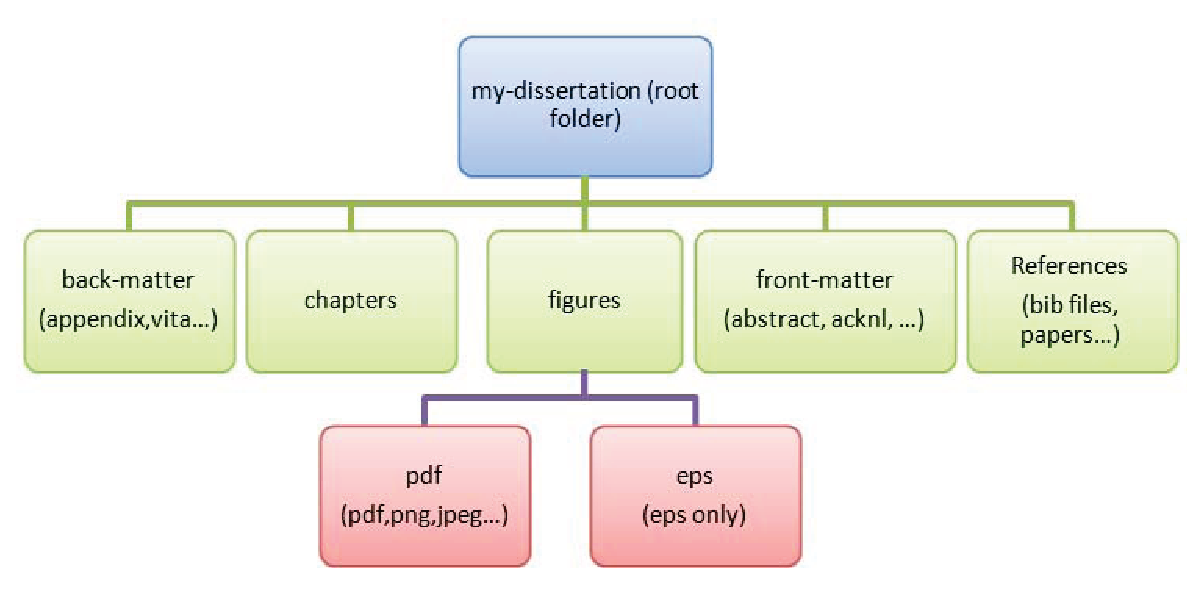
\includegraphics[width=6.5in]{fig01-folder-structure}\\
  \caption{UT thesis template folder structure.}\label{fig:intro-folder-structure}
\end{figure}
The general structure of this template is based on the tree shown in Figure \ref{fig:intro-folder-structure}. The titles of the folders are self descriptive and should guide you to proper file placement. Note that this is only a suggested model that could be modified to fit your own organizational structure.

There are two important files in this template: ``my-dissertation.tex'' and ``utthesis.cls''. The ``utthesis.cls'' is the class file that contains the settings, definitions, packages, and macros for this template to work properly and is located in the root directory. This file constitutes the document class for the template. It is based on the report class and provides some customized functionality. It will also generate a title page for you. In certain cases, one of the packages included in this template may conflict with a package that you are adding. You will have to resolve this conflict by either removing the package that is not being used or by modifying some settings with either packages. The packages that are preloaded in this class file are: amsmath, amsthm, amssymb, setspace, geometry, hyperref, and color.

The ``my-dissertation.tex'' file is the main file for your thesis/dissertation. This is where you bring all of the pieces together. Each individual section of your dissertation should be its own .tex file saved in the proper place. For example, a chapter for your dissertation should be saved in the ``chapters" folder. Whereas your acknowledgments file should be saved in the ``front-matter" folder. The ``my-dissertation.tex" file is the file you compile to make your dissertation. It'll call all of the included files and compile the document properly. You may want to change the name of the file to something like ``my-name-dissertation.tex''. Next, invoke the proper options for the ``utthesis'' document class. This class will take all the options for the report class in addition to two options: thesis/dissertation and monochrome. If you are writing a thesis, you must use "thesis" otherwise, use "dissertation" or omit that option because dissertation is the default setting. The monochrome option converts all your document to monochrome - except figures. This is very useful when printing your document. Because this dissertation has colored hyperlinks, these will look washed out when printed on a monochrome printer. Therefore, it is handy to have a monochrome copy of your thesis for print. 

Now you are ready to fill in the proper values corresponding to your title, name, degree, etc. This can be done in the following section:
\begin{verbatim}
%%%%%%%%%%%%%%%%%%%%%%%%%%%%%%%%%%%%%%%%%%%%%%%%%%%%%%%%%%%%%%%%%%%%%%%%%%%%
% TO DO: FILL IN YOUR INFORMATION BELOW - READ THIS SECTION CAREFULLY
%%%%%%%%%%%%%%%%%%%%%%%%%%%%%%%%%%%%%%%%%%%%%%%%%%%%%%%%%%%%%%%%%%%%%%%%%%%%
\title{My Thesis or Dissertation Title}	 % title of thesis/dissertation
\author{Smokey Volunteer}                % author's name
\copyrightYear{2017}            		 		      % copyright year of your 
                                           thesis/dissertation
\graduationMonth{May}           	     	  % month of graduation for your 
                                           thesis/dissertation
\degree{Doctor of Philosophy}   % degree: Doctor of Philosophy, Master of 
                                  Science, Master of Engineering...
\university{The University  of Tennessee, Knoxville}	% school name
%%%%%%%%%%%%%%%%%%%%%%%%%%%%%%%%%%%%%%%%%%%%%%%%%%%%%%%%%%%%%%%%%%%%%%%%%%%%
\end{verbatim}

\section{References}
The bibliography style used in this template is "apalike". It is an author-year style based on the APA specification. Here are a few examples. T. Hungerford wrote a book on Algebra, \citep{Hungerford1974}. In 1999, D. F. Anderson and P. S. Livingston wrote the defining paper on zero-divisor graphs of commutative rings in \citep{AndersonLivingston1999}. You can also point out specific theorems in papers, such as the fact that the zero-divisor graph always has diameter less than or equal to $3$, \citep[Theorem 2.3]{AndersonLivingston1999}. You can also list several references at once. For example, for more on zero-divisor graphs see \citep{AAS2011,AFLL2001}. However, you can change this style to any format you'd like. The code in the ``my-dissertation.tex" file is 
\begin{verbatim}
\utbiblio{#1}{apalike}{references-dissertation}
\end{verbatim} 
The first entry (``\#1") must remain there. It deletes the title ``Bibliography" from being printed again at the top of the bibliography page. The title ``Bibliography" should only appear on the title page. The second entry can be changed to any natbib style you'd like. For example, plainnat, humannat, etc. The third entry is the name of your bibliography .tex file. Remember to run BibTeX in order to compile the bibliography correctly. For more information, visit \href{http://merkel.texture.rocks/Latex/natbib.php}{http://merkel.texture.rocks/Latex/natbib.php}.

\section{Theorem environments}
This template contains predefined theorem, lemma, proposition, corollary, and definition environments. For example,
\begin{definition}
	This is your definition.
\end{definition}
\begin{proposition}
	This is an example of a proposition.
\end{proposition}
\begin{theorem}[First theorem]\label{thm:theorem-a}
    This is an example theorem.
\end{theorem}
\begin{proof}[Proof for theorem]
    This is the proof for this theorem.
\end{proof}
\begin{lemma}[First lemma]
    This is the first lemma.
\end{lemma}
\begin{proof}
	This is the proof for this lemma that requires Theorem \ref{thm:theorem-a}.
\end{proof}
\begin{corollary}
    This is the first corollary.
\end{corollary}

\section{Figures and Tables}
\subsection{General Rules}
To comply with the 2017 dissertation formatting, figure captions should be placed below the figure and table captions should be placed above the table. Also, if a table or figure takes up more than half the page, then there should be no text on that page (except for the caption of course). Lastly, you must allow tables and figures to float. DO NOT HARD CODE POSITIONS. In addition, no table or figure should go into the margins. If a table or figure does creep into the margins you can either resize it so that it properly fits within the margins, or put it on its own page and make that specific page landscape. See Figure \ref{fig:wide-pic} for an example. Note the page number location in the example. The code for this is given by:

\begin{verbatim}
\begin{landscape}
\thispagestyle{mylandscape}
	\begin{figure}[h]
		\centering
		\includegraphics[width=9in]{32303-TheHill-byJoshQueener.jpg}
		\caption{This view of The Hill is too wide for a portrait page.}
		\label{fig:wide-pic}
	\end{figure}
\end{landscape}
\end{verbatim}

Be careful about where you place this landscape page, as well as all figures and tables. These objects are not considered part of the text, and thus their placement should not be assigned to a precise location. The general rule to follow is that no text page should have significant white space, with the exception being the last page of a chapter. So if you mention a figure in some paragraph but the figure will not fit on the remainder of the page, continue the text (even if it's a new section) to fill the current page with text and then place the figure on the next page. To see an example of this, consider this page you are reading now. We've mentioned Figure \ref{fig:wide-pic} in the previous paragraph. However, it requires a new page and since there is plenty of space on this page, we've filled it with text and delayed the \verb|\begin{landscape}| section of code until the appropriate position.

\subsection{Single figures}
For more information, check out the following page: \\ \href{http://en.wikibooks.org/wiki/LaTeX/Floats,_Figures_and_Captions}{http://en.wikibooks.org/wiki/LaTeX/Floats,\_Figures\_and\_Captions}
\begin{verbatim}
    \begin{figure}[t for top, b for bottom, h for here]
        % Requires \usepackage{graphicx}
        \centering % center the figure
        \includegraphics[width=5in or 127mm etc...]{figure-name}\\
        \caption{figure caption}\label{figure label}
    \end{figure}
\end{verbatim}

\begin{figure}[h]
  \centering
  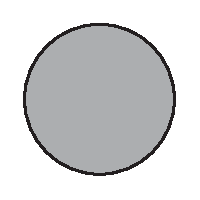
\includegraphics[width=3in]{fig02a-circle}\\
  \caption{Sample caption.}\label{label}
\end{figure} 

\subsection{Multipart figures}
For multipart figures, you need to use the package "subfig". here's an example:
\begin{verbatim}
\begin{figure}[h]
   \centering
   \subfloat[Circle]{\label{fig:figure-a}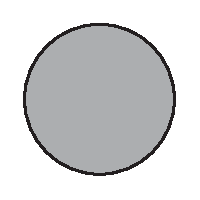
\includegraphics[width=1.1in]
     {fig02a-circle}}
   \subfloat[Rectangle]{\label{fig:figure-b}
\includegraphics[width=1.1in]
     {fig02b-rectangle}}
   \subfloat[Cube]{\label{fig:figure-c}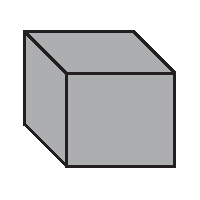
\includegraphics[width=1.1in]
     {fig02c-cube}}
   \caption{Geometric shapes.}
   \label{fig:multipart-figure}
\end{figure}
\end{verbatim}
\begin{figure}[h]
        \centering
        \subfloat[Circle]{\label{fig:figure-a}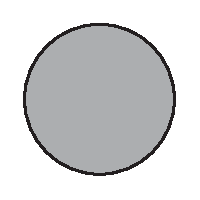
\includegraphics[width=1.1in]{fig02a-circle}}
        \subfloat[Rectangle]{\label{fig:figure-b}
\includegraphics[width=1.1in]{fig02b-rectangle}}
        \subfloat[Cube]{\label{fig:figure-c}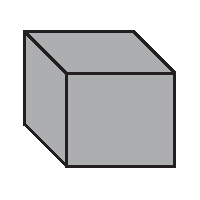
\includegraphics[width=1.1in]{fig02c-cube}}
        \caption{Geometric shapes.}
        \label{fig:multipart-figure}
\end{figure}
To add some space between the figures above, one can use the usual spacing commands such as ``\verb|\qquad|''. For example, 
\begin{verbatim}
\begin{figure}[h]
   \centering
   \subfloat[Circle]{\label{fig:fig-a-space}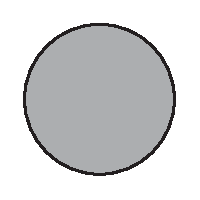
\includegraphics[width=1in]
     {fig02a-circle}} \qquad
   \subfloat[Rectangle]{\label{fig:fig-b-space}
\includegraphics[width=1in]
     {fig02b-rectangle}}\qquad
   \subfloat[Cube]{\label{fig:fig-c-space}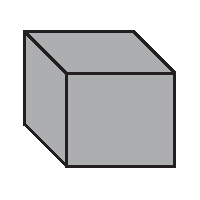
\includegraphics[width=1in]
     {fig02c-cube}}\qquad
   \caption{Geometric shapes with space between images.}
   \label{fig:multipart-figure-space}
\end{figure} 
\end{verbatim}

\begin{figure}[h]
        \centering
        \subfloat[Circle]{\label{fig:fig-a-space}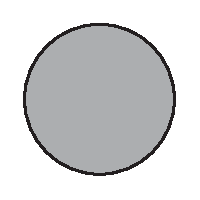
\includegraphics[width=1in]{fig02a-circle}} \qquad
        \subfloat[Rectangle]{\label{fig:fig-b-space}
\includegraphics[width=1in]{fig02b-rectangle}}\qquad
        \subfloat[Cube]{\label{fig:fig-c-space}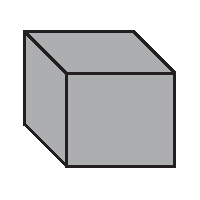
\includegraphics[width=1in]{fig02c-cube}}\qquad
        \caption{Geometric shapes with space between images.}
        \label{fig:multipart-figure-space}
\end{figure} 

\begin{landscape}
\thispagestyle{mylandscape}
	\begin{figure}[h]
		\centering
		\includegraphics[width=9in]{32303-TheHill-byJoshQueener.jpg}
		\caption{This view of The Hill is too wide for a portrait page.}
		\label{fig:wide-pic}
	\end{figure}
\end{landscape}

\subsection{Tables}
Again, table captions should be placed above the table. See Table \ref{tab:table-a} for an example and to learn about Smokey's history\footnote{According to Wikipedia: \href{https://en.wikipedia.org/wiki/Smokey_(mascot)}{https://en.wikipedia.org/wiki/Smokey\_(mascot)}}. For more information about tables, see \href{https://en.wikibooks.org/wiki/LaTeX/Tables}{https://en.wikibooks.org/wiki/LaTeX/Tables}.

\begin{table}[hb]
\caption{Smokey's History}
\label{tab:table-a}
\begin{center}
\begin{tabular}[b]{|c|c|c|c|}
	\hline
	Dog & Years & Record & Pct. \\ \hline
	Blue Smokey & 1953-1954 & 10-10-1 & .500 \\ \hline
	Smokey II & 1955-1963 & 58-39-5 & .597 \\ \hline
	Smokey III & 1964-1977 & 105-39-5 & .729 \\ \hline
	Smokey IV & 1978-1979 & 12-10-1 & .545 \\ \hline
	Smokey V & 1980-1983 & 28-18-1 & .608 \\ \hline
	Smokey VI & 1984-1991 & 67-23-6 & .744 \\ \hline
	Smokey VII & 1992-1994 & 27-9 & .750 \\ \hline
	Smokey VIII & 1995-2003 & 91-22 & .805 \\ \hline
	Smokey IX & 2004-2012 & 62-53 & .539 \\ \hline
	Smokey X & 2013-present & 21-17 & .552 \\ \hline
\end{tabular}
\end{center}
\end{table}



    \chapter{Background of Electrochemical Reprocessing} \label{ch:background}

The United States currently has approximately 70000 MTU of spent nuclear fuel (SNF) sitting either in intermediate length storage via spent fuel casks (heavily shielded concrete containers), or in spent fuel pools [insert CURIE citation here]. Most reactor sites are at or near their limit for pool storage, and above ground cask storage is becoming commonplace. The United States has responsibility for commercially produced spent nuclear fuel, per 10 CFR 961.11, listed below [insert 10 CFR citation]. \\

\begin{lstlisting}
Witnesseth that:

Whereas, the DOE has the responsibility for the disposal of spent nuclear fuel and high-level radioactive waste of domestic origin from civilian nuclear power reactors in order to protect the public health and safety, and the environment; and

Whereas, the DOE has the responsibility, following commencement of operation of a repository, to take title to the spent nuclear fuel or high-level radioactive waste involved as expeditiously as practicable upon the request of the generator or owner of such waste or spent nuclear fuel; and

Whereas, all costs associated with the preparation, transportation, and the disposal of spent nuclear fuel and high-level radioactive waste from civilian nuclear power reactors shall be borne by the owners and generators of such fuel and waste; and

Whereas, the DOE is required to collect a full cost recovery fee from owners and generators delivering to the DOE such spent nuclear fuel and/or high level radioactive waste; and

Whereas, the DOE is authorized to enter into contracts for the permanent disposal of spent nuclear fuel and/or high-level radioactive waste of domestic origin in DOE facilities; and

Whereas, the Purchaser desires to obtain disposal services from DOE; and

Whereas, DOE is obligated and willing to provide such disposal services, under the terms and conditions hereinafter set forth; and

Whereas, this contract is made and entered into under the authority of the DOE Organization Act ( Pub. L. 95-91, 42 U.S.C. 7101et seq.) and the Nuclear Waste Policy Act of 1982 ( Pub. L. 97-425, 42 U.S.C. 10101et seq.)

\end{lstlisting}

As such, the United States is currently investigating a number of possible solutions for spent nuclear fuel. The most widely known route is via direct disposal at a facility such as Yucca Mountain. This route would involve simply taking the spent fuel at reactor sites, repackaging it, and then disposing of it in a geologic repository. Some consider this route to be wasteful, not utilizing the full potential of nuclear fuel. The reason for this is that spent fuel is composed of $\approx 96\%$ uranium [insert world-nuclear citation], and reprocessing the SNF would offer multiple benefits. \\

\section{Reprocessing}
The first benefit is utilization of more of the potential energy of the nuclear fuel. Reprocessing the fuel allows the majority of the uranium to be used as fuel a second time, if also using fast spectrum reactors. A second benefit is the reduced amount of SNF, both in terms of total mass, and potentially, heat volume, that would be going to a repository. \\
\subsection{PUREX}
The United States has been reprocessing SNF since the Manhattan project, although not for the purpose of recycling commercial fuel. The United States has used the Plutonium Uranium Solvent Extraction (PUREX) process for decades to recover plutonium from specially burned nuclear fuel for the purpose of harvesting nuclear weapons material. This process involves multiple steps of reducing and oxidizing the uranium and plutonium, to produce an immiscible mixture, whereby uranium and plutonium are selectively extracted using compounds such as TBP to aid in extraction. This process is well understood, and there is significant experience with it. However, there are drawbacks. A significant amount of byproduct nuclear waste is produced via this method, and it can not be used on very fresh SNF, as there are heat limits to this technique. It is also not suitable to sodium bonded fuel [insert Argonne citation]. The last drawback is the large footprint required for a PUREX facility. \\
\subsection{Pyroprocessing}
An alternative method of reprocessing that has been proven to work is electrochemical reprocessing, also known as pyroprocessing. This method utilizes the fact that the Gibbs Free Energy of uranium, plutonium, and other transuranics have slight differences, and as such can be separated via adjusting the voltage going through a molten salt mixture. The process of pyroprocessing, of which the safeguards is the subject of this thesis, is described as follows. \\ % I don't like how this last sentence is worded.

\begin{figure}[h]
  \centering
  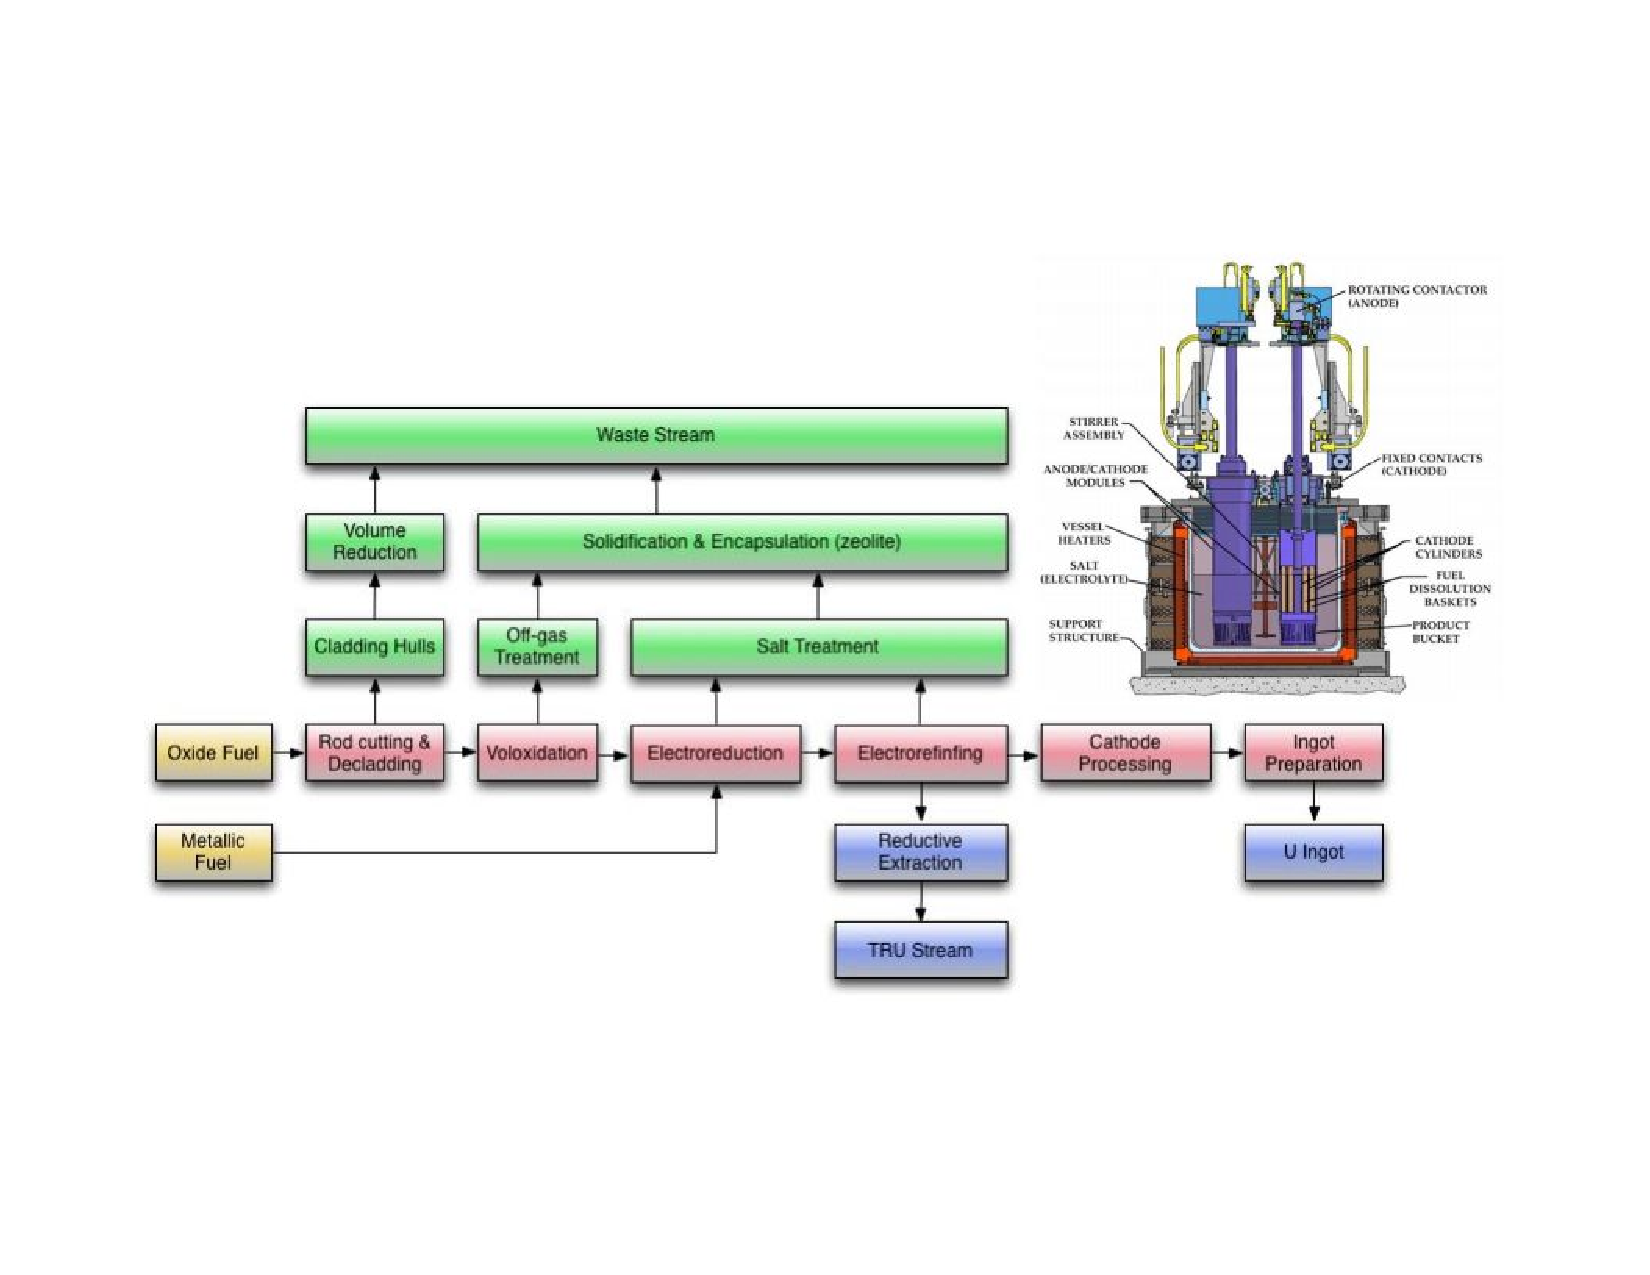
\includegraphics[width=15cm]{Pyroprocessing_Description_Skutnik.pdf}\\
  \caption{Flow sheet illustrating the pathways of pyroprocessing.}\label{pyro_flow}
\end{figure} 

\newpage

\subsection{Fuel Rod Processing}
As Figure \ref{pyro_flow} shows, the process starts with the spent fuel rods being extracted and then being chopped. The fuel pellets are then extracted, and sent to the voloxidizer, if it is not already in metallic form. The zirconium cladding fuel rod cladding is sent for metal waste disposal. This part is completely mechanical. The fuel pellets will then need to be oxidized via voloxidation. 

\subsection{Voloxidation}

Voloxidation serves two purposes: the first is to release and capture some of the fission gasses, and the second is to prepare the oxide fuel for electroreduction. Voloxidation is performed by flowing oxygen through a voloxidation reactor, producing the following reaction.

\begin{equation}
3UO_2 + O_2 \rightarrow U_3O_8
\end{equation}

The result of this is that the fuel material is converted to a less dense, higher surface area powder to be sent to electroreduction. Several items of note for this process are the air flow rate and the temperature of the system. The oxygen flow rate should be such that it produces the oxidizing reaction without being so high as to carry off fuel particles into the off gas stream. The temperature must be maintained above 500 $^{\circ}$C and below 1000 $^{\circ}$C. Temperatures above 1000 $^{\circ}$C can cause undesirable sintering of particles. An interesting item to note, is that the voloxidation process results in elimination of a fraction of the fission products. It eliminates the majority of the technetium and ruthenium, while elminating between $\frac{1}{5}$ to $\frac{1}{3}$ of the cesium.


\subsection{Electroreduction}

After the material has been pulverized and converted to $U_3O_8$, the material must then be electroreduced, to yield pure metalic material, rather than an oxide. The electrolyte used is $LiCl-Li_2O$ at 650 $^{\circ}$C, with a platinum rod anode. The cathode of this cell is the fuel powder, contained within a magnesia membrane walls, so ions can traverse the membrane to react. The reaction that takes place is shown below. \\ 

\begin{equation}
Li^+ + e^- \rightarrow Li
\end{equation}

\begin{equation}
M_xO_y + 2yLi \rightarrow xM + yLi_2O
\end{equation}

Some of the fission products such as cesium and barium (alkaline elements) will dissolve into the salt as metal chlorides, as it is electrochemically favorable for them to do so. These fission products can be disposed of when the salt is treated. The electroreduction process is extremely effective, reducing uranium and plutonium to metals at rates of $\approx$ 99 and 96 \%, respectively. The salt then has to be separated from the transuranic metals. This is done by evaporation at temperatures of around 1200 $^{\circ}$C. During this process, some actinides can be contained in the waste streams of fission products and salt. \\

\subsection{Electrorefiner}
 It is then inserted into a basket to be placed into the electrorefiner. At the electrorefiner, the fuel is dissolved into the molten salt with an applied voltage. The voltage applied will pull off components of the fuel in a particular order, corresponding to the Gibbs Free Energy. The lathanides will dissolve into the salt first, then the  uranium and transuranics will go into the salt. The noble metals (iron, zirconium, cadmium, etc) will stay in the chopped fuel basket, as they have higher Gibbs Free Energy. After uranium and transuranics are dissolved into the salt, the voltage is then lowered, allowing the reaction to proceed in reverse. The uranium will plate out first as dendrites on the solid cathode. After uranium collection on the solid cathode has saturated, the voltage is lowered again, this time pulling out the transuranics, along with some of the residual uranium, into a liquid cadmium cathode. After these two steps, the cathodes are sent off to collect the uranium and transuranics, eventually producing solid metal ingots. \\

The salt will over time accumulate fission products and trace amounts of uranium and transuranics. Every so often, the salt must be purified, with the fission products being captured in zeolite for storage/disposal. Throughout this process, whenever possible, off-gasses (such as tritium and xenon) are captured for disposal. \\

\section{Hybrid K-Edge Densitometry}

\subsection{Description of HKED}

Hybrid K-Edge densitometry is a nuclear safeguards technique that is based on two separate techniques k-edge densitometry (KED) and x-ray fluorescence (XRF), and combines them together into one measurement device. This technique has been proven to work for aqueous based reprocessing, and is scheduled to be used in the Rokkasho reprocessing facility in Japan [cite Rokkasho paper IAEA]. \\

K-edge densitometry works by using the fact that the mass attenuation coefficient for gamma rays encounters a significant increase around electron shells. In particular, the k-shell is of interest for several reasons. The first is that it is located at 115.6 keV, and is very noticeable. The second is that the mass attenuation coefficient for the k-edge is a very sharp, distinct rise and fall. These two factors combine to make for a very clean and easy measurement. \\

The k-edge drop occurs when a gamma ray passes through a material, such as molten salt, and encounters uranium. To perform this measurement, a gamma ray source is shown at a molten salt sample, with a detector behind the sample. Gamma rays interact more strongly with high atomic number material, so in the abscence of uranium, there is negligible gamma ray intensity drop at the 115.6 keV energy on a gamma detector. However, as uranium concentration in the salt is increased, a noticeable decrease in gamma ray intensity occurs around 115.6 keV in the detector pulse height spectrum. This is due to the uranium mass attenuation coefficient at 115.6 being significantly higher than the nearby energies, and blocking transmission of gammas at that energy. Plutonium's k-edge is located at 121.8 keV [cite los alamos].\\

X-ray fluorescence occurs as a result of the ejection of k-shell electrons due to photon interaction. This electron ejection causes a higher orbit electron to fall and take the vacant spot, emitting a characteristic x-ray. A list of common x-rays emitted from uranium and plutonium k-shell ejections is listed in \ref{xrays-uranium-plutonium} [cite Matt's Dissertation]. \\

\begin{table}[hb]
\caption{X-ray Energies Emitted By Uranium and Plutonium K-shell Ejections (keV)}
\label{xrays-uranium-plutonium}
\begin{center}
\begin{tabular}[b]{|c|c|c|c|c|c|c|}
	\hline
	Element & $K_{\alpha1}$ & $K_{\alpha2}$ & $K_{\beta1}$ & $K_{\beta2}$ & $K_{\beta3}$ & $K_{\beta4}$\\ \hline
	Uranium & 98.43 & 94.65 & 111.3 & 114.5 & 110.4 & 114.8 \\ \hline
	Plutonium & 103.7 & 99.52 & 117.2 & 120.6 & 116.2 & 120.9\\ \hline

\end{tabular}
\end{center}
\end{table}

Using a combination of these two techniques, it is possible to determine the concentration of elements such as actinides in the salt. 




    \chapter{Methods}\label{ch:methods}
This chapter will cover the approach taken to implement HKED safeguards into the SSPM. An introduction to the ORIGEN modeling of spent fuel will be the first step, then an introduction to the MCNP model will be the second topic. This will be followed by methods used to decrease runtime and automate generation of the MCNP simulations.


\section{Used Fuel Source Terms}
Spent nuclear fuel is primarily composed of very lightly enriched uranium, with around 5\% fission products, and 1-2\% plutonium. However, burnup, length of operating cycles, downtimes between cycles, and original fuel enrichment, among other factors, can cause the isotopics of spent fuel to vary from one discharge to another. This implies that using a single spent fuel composition for HKED modeling could be misrepresentative, and lead to incorrect KED k-edge drops, for example. To rectify this, the first part of this project was to identify common spent fuel enrichments and burnups. This was based off of a Los Alamos National Laboratory emperical relationship [insert citation], relating burnup to original enrichment. \\

It is beneficial to describe the ORNL SCALE code before continuing. SCALE is, among other things, a reactor physics code which includes multiple sub-packages. One of these packages is the Oak Ridge Isotope Generation (ORIGEN) code. This code solves the Bateman equations to handle depletion cases for nuclear fuel. This code allows researchers to predict discharge isotopic compositions based off of reactor power, cycle length, and downtimes. \\

Once the space of enrichment and burnup values was determined, a Python script was written by Jonathan Mitchell and Steven Skutnik to automate production of ORIGAMI (an alternative input format to ORIGEN) input decks. A change that was made to this script by Michael Cooper was to switch the reactor cycle lengths and number of cycles from the original 12 months and 5 cycles, to the values of 18 months and 3 cycles. This change was based on the fact that the United States reactors typically operate on 18 month cycles [insert MIT and EPRI references]. The Python ORIGAMI generation script was then used to generate the ORIGEN input to use in the SCALE. \\

The range of burnups was restricted to the low point of 20 GWd/MTU, and high point of 60 GWd/MTU. This were chosen based off of typical US spent fuel composition, assuming an average burnup of 45 GWd/MTU. Fuel rods on the edges of reactors will not have as high of burnup due to reactor operators optimizing the reactor neutronics, and could have values significantly lower than the average 45 GWd/MTU. Values below 20 GWd/MTU are typically reserved for special cases such as research reactors or weapons material generation [insert weapons reference]. Values above 60 GWd/MTU typically don't occur in the US due to the fuel generating neutron poisons over time and depleting the U-235 in the fuel. \\

With this in mind, the enrichment and burnup values chosen for the spent fuel source terms are listed in Tables \ref{source1} and \ref{source2}. \\



\begin{table}[p!]
\caption{Spent Fuel Compositions For Source Terms}
\label{source1}
\begin{center}
\begin{tabular}[b]{|c|c|c|}
	\hline
	Burnup $\frac{GWd}{MTU}$ & Enrichment & Cooling Time (Years)\\ \hline
	20 & 1.96\% & 5 \\ \hline
	20 & 1.96\% & 15 \\ \hline
	20 & 2.17\% & 5 \\ \hline
	20 & 2.17\% & 15 \\ \hline
	20 & 2.39\% & 5 \\ \hline
	20 & 2.39\% & 15 \\ \hline
	25 & 2.26\% & 5 \\ \hline
	25 & 2.26\% & 15 \\ \hline
	25 & 2.51\% & 5 \\ \hline
	25 & 2.51\% & 15 \\ \hline
	25 & 2.76\% & 5 \\ \hline
	25 & 2.76\% & 15 \\ \hline
	30 & 2.55\% & 5 \\ \hline
	30 & 2.55\% & 15 \\ \hline
	30 & 2.83\% & 5 \\ \hline
	30 & 2.83\% & 15 \\ \hline
	30 & 3.11\% & 5 \\ \hline
	30 & 3.11\% & 15 \\ \hline
	35 & 2.81\% & 5 \\ \hline
	35 & 2.81\% & 15 \\ \hline
	35 & 3.13\% & 5 \\ \hline
	35 & 3.13\% & 15 \\ \hline
	35 & 3.44\% & 5 \\ \hline
	35 & 3.44\% & 15 \\ \hline


\end{tabular}
\end{center}
\end{table}



\begin{table}[p!]
\caption{Spent Fuel Compositions For Source Terms (continued)}
\label{source2}
\begin{center}
\begin{tabular}[b]{|c|c|c|}
	\hline
	Burnup $\frac{GWd}{MTU}$ & Enrichment & Cooling Time (Years)\\ \hline
	40 & 3.07\% & 5 \\ \hline
	40 & 3.07\% & 15 \\ \hline
	40 & 3.41\% & 5 \\ \hline
	40 & 3.41\% & 15 \\ \hline
	40 & 3.75\% & 5 \\ \hline
	40 & 3.75\% & 15 \\ \hline
	45 & 3.31\% & 5 \\ \hline
	45 & 3.31\% & 15 \\ \hline
	45 & 3.68\% & 5 \\ \hline
	45 & 3.68\% & 15 \\ \hline
	45 & 4.05\% & 5 \\ \hline
	45 & 4.05\% & 15 \\ \hline
	50 & 3.55\% & 5 \\ \hline
	50 & 3.55\% & 15 \\ \hline
	50 & 3.94\% & 5 \\ \hline
	50 & 3.94\% & 15 \\ \hline
	50 & 4.34\% & 5 \\ \hline
	50 & 4.34\% & 15 \\ \hline
	55 & 3.77\% & 5 \\ \hline
	55 & 3.77\% & 15 \\ \hline
	55 & 4.19\% & 5 \\ \hline
	55 & 4.19\% & 15 \\ \hline
	55 & 4.61\% & 5 \\ \hline
	55 & 4.61\% & 15 \\ \hline
	60 & 3.99\% & 5 \\ \hline
	60 & 3.99\% & 15 \\ \hline
	60 & 4.44\% & 5 \\ \hline
	60 & 4.44\% & 15 \\ \hline
	60 & 4.88\% & 5 \\ \hline
	60 & 4.88\% & 15 \\ \hline

\end{tabular}
\end{center}
\end{table}


Now that the source term generation has been described, a discussion of the HKED MCNP model is next. \\

\section{MCNP Modeling of HKED}

\subsection{MCNP Model}
A MCNP model was constructed by former UT PhD student Matt Cook as part of his dissertation project. This model contains the geometries needed to properly describe a HKED measurement apparatus such as the one shown in Figure \ref{HKED-apparatus}. This MCNP model works by performing two stage simulations for KED and XRF scenarios separately. Since the measurements are not interdependent, this allows for the KED and XRF to be handled separately for simulation, then the results can later be collaborated. This aids in the ease of building and troubleshooting the model [cite Matt dissertation]. \\


\begin{figure}[h]
  \centering
  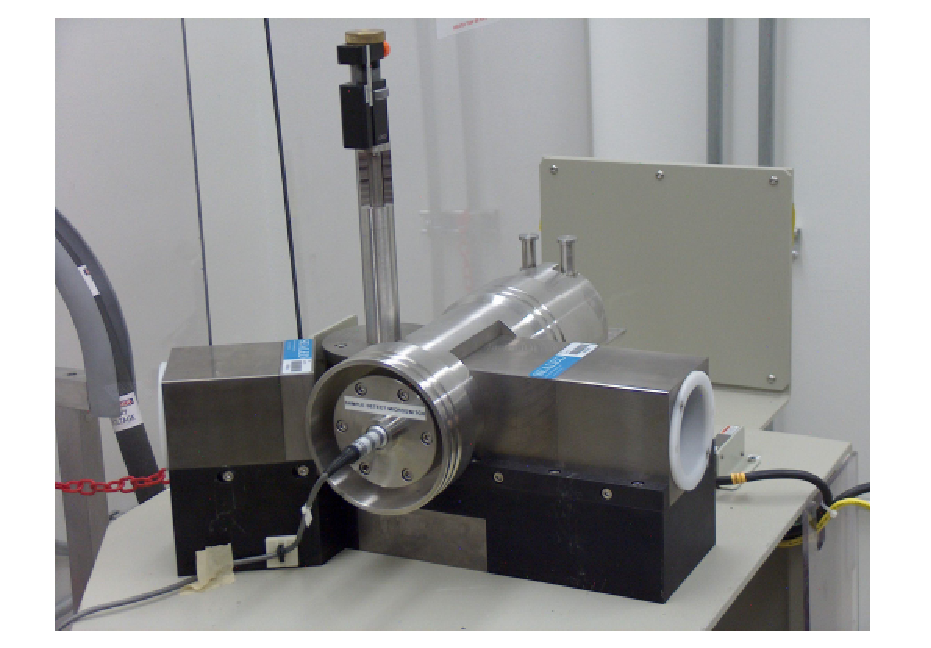
\includegraphics[width=15cm]{HKED_Apparatus.pdf}\\
  \caption{HKED system without outer lead shielding. Both XRF (left) and KED (right) component beamlines are exposed and germanium detectors have been removed [cite Matt dissertation]}
 \label{HKED-apparatus}
\end{figure} 


When the model was received by Michael Cooper, there was minimal instruction on how to use the model.  The first step of this project was to recover the knowledge needed to run the MCNP model, as it had been over a year since it had been developed, and Matt Cook, the only person with intimate knowledge of using the model at the time, was working on a different task after his graduation. To this goal, the model was thoroughly reviewed, along with review of Cook's dissertation, to reveal the folllowing method of operation. \\

The model operates on several principles. The first is that the model uses 2 stages. The stage 1 simulations are used to generate gamma energy distributions exiting the beamline, which are to be used for the source file for the stage 2 simulations. The stage 2 simulations determine the pulse height response using F8 tallies. This effectively means that the stage 1 simulations guide the stage 2 simulations by building a more focused gamma source term  exiting the beamline that is going from the salt sample to the detector [cite Matt dissertation]. \\ % last sentence needs reworded as it is a run-on

\subsection{Preliminary Work Performed On Model}

The first step that was done with the MCNP model to get it operating properly was to simply run it as is, and check the output. The first version of the model used was the KED version, as it was the easier of the two to converge statistically. The stage 1 model was ran, the results processed and a source term output generated, then the stage 2 ran. The output of the stage 2 pulse height tally, however, did not match the published results from Cook's dissertation, even when using an identical fuel/salt mixture. After discussion with Skutnik and Cook, it was realized that the Cd-109 source term that was used for normalization in Cook's dissertation results was not being included, due to using the incorrect version of the stage 1 postprocessing script. After the correct version was used (along with modifications to the script to properly reference the correct MCNP surfaces), a compareable pulse height spectra was obtained for the sample case of EBR fuel using the stage 2 simulation output. \\

For the XRF version of the model, the first step again was to simply run the model as it was given. The results of the stage 2 XRF simulations, however, revealed a very jagged pulse height spectrum, with very high uncertainty. The next step was to inspect the stage 1 output, where it was realized that extremely few particles were actually reaching the F2 tally used to generate the gamma source term for the stage 2 simulation. Simulations were then ran increasing the number of stage 1 particles ran, but this did not make an appreciable difference in the number of particles reaching the F2 tally. Following this, a review was done of the variance reduction that was implemented in the model. It was determined that the DXTRAN variance reduction had been commented out in the model that was given, which resulted in extremely few particles reaching the F2 tally. To rectify this, the proper DXTRAN was turned on around the stage 1 F2 tally, and the model was run again. This time, the trial runs produced results that matched those published in Cook's dissertation. \\

The overall variance reduction techniques employed in the XRF model were as follows [cite Matt dissertation].
\begin{enumerate}
\item Forced collisions: All particles entering the sample are required to interact and weighted appropriately
\item MCNP DXTRAN Sphere: Particles are forced to travel to the sphere volume, and are weighted appropriately
\item Spatial weight window mesh: Particles are weighted and controlled via splitting and Russian roulette based on position
\item Energy weight window mesh: Particles are weighted and controlled via splitting and Russian roulette based on energy
\end{enumerate}

\subsection{Generation of MCNP Outputs for Modeling}

It was determined that to properly model the k-edge drop and x-ray fluorescence peaks, a relatively large number of MCNP runs with acceptable statistical convergence would be needed. To accomplish this, 54 MCNP runs were done for the stage 1, and then 54 for the stage 2 simulations, with this being done for both KED and XRF. A total of 216 MCNP simulations were ran. These are based on \ref{source1} and \ref{source2}. \\

The first step for the KED aspect of the MCNP model is to find the total mass fraction of actinides. Then using the Python script Convert\_Origen.py, the ORIGEN output is imported to Python. The elemental composition of the spent fuel source term from ORIGEN is determined in the form of mass percents. These mass percents are then proportionately assigned to the MCNP model's total mass percentage of fuel in the salt, replacing the default values of EBR spent fuel with commercial spent fuel mentioned in Tables \ref{source1} and \ref{source2}. Typical values of total fuel mass percent of the salt are around 7\%, with 6.8\% of the salt fuel mixture's mass percent being uranium, and plutonium making up the majority of the remainder. This convention of mass percents follows one of the two methods to specify to MCNP the percentage of elements in each material used in the model. Of note, for commercial spent fuel, there is an extremely small presence of any actinides other than uranium and plutonium, with uranium being vastly more abundant than plutonium. This will cause the plutonium k-edge drop to be barely visable. \\ % This needs reworded: it assumes the reader is familiar with MCNP mass percentage convention, and without MCNP knowledge, this paragraph isn't readable.

After the mass percentages of the materials in the MCNP input decks are corrected, the stage one simulations can be ran in sequence. This was done via batch scripting on a local computer built to handle moderately large MCNP tasks. A total of 250 million particles were ran for each stage 1 run, requiring approximately 2.5 hours per each simulation on a core i7 8700. The more particles that are ran, the better the stage 1 energy source file that is generated will be, however, increasing the number of particles increases runtime proportionately, while uncertainty is proportional to ${N^{-0.5}}$. This states that in order to reduce uncertainty by a factor of 10, the number of particles must be increased by a factor of 100. As such, there is an optimization between runtime and acceptable uncertainty. \\

Once the 54 stage 1 simulations are complete, they are then put through a Python postprocessing script that Matt Cook wrote, to extract and write the energy source files to be used in the stage 2 simulations. The stage 2 simulations are then ran, again via batch script, to get the final detector response results that are desired. For the stage 2 simulations, 100 million particles are used, and the run time is typically around 2.5 hours. \\

After the completion of the the stage 2 simulations are complete, the MCNP output file is then processed by the Python script Spectra\_Retrieve.py. This script searches the MCNP output for the F8 tally results, and converts them from the text file they are supplied in to a more usable .csv file. This facilitates importing of the spectra that were simulated into a Python script for emperically modeling the k-edge drop. \\

A similar approach is followed for the XRF version of the model, however, the XRF requires significant variance reduction. Without multiple methods of variance reduction, the XRF version of the model requires trillions of particles to converge, with unrealistic runtimes. The variance reduction employed was described in the section on preliminary work with the model. \\

\subsection{Potential Issues With MCNP Modeling}

The overall task of modeling HKED with MCNP works very well. However, due to MCNP's Monte Carlo nature, there are a few issues. The first is statistical uncertainty, and the second is "particle hanging". \\

For the HKED models, both KED and XRF, the uncertainty listed in the output of the S2 tally is not necessarily correct. This is because of the way the simulation works. The S1 simulation guides the particles to the entrances of the beamlines, where a F2 tally is waiting to generate a source term for the S2 simulation. Therefore, there is intrinsic uncertainty in the S2 source term, resulting from the S1 simulation results. In a sence, since the S1 simulations are guiding the S2 simulations, if the S1 simulation has an ultra large uncertainty, it can misguide the source term energy distribution used by the S2 simulations. This will not be reflected in the output of the S2 F8 tally, as it is only concerned with particles traveling from the beamline to the microcell target, without any care for how many particles actually reach the beamline. In reality, extremely few particles (on the order of typically less than 10) reach each energy channel for the S1 tally, causing extremely high variance. As a result, even though the S2 MCNP output will list uncertainties on the order of 1-5\% for KED, and less than 1\% for XRF, these values should be taken with a grain of salt, as they can be very misleading. However, with regards to reliability of the model to accurately reproduce HKED spectra, this is assumed to be true, based on benchmarking of HKED data done by Cook. As of now, the assumption will be that both the KED and XRF simulations model the spectra to within 5\% as the S2 results indicate. \\

Regarding particle hanging, what is being referred to is an anomaly within Monte Carlo. Usinng Monte Carlo, it is theoretically possible for a particle to never terminate, and thus for a program such as MCNP to require infinite time to track a particular particle. This is extraordinary rare for normal MCNP simulations, however, when running simulations with extensive variance reduction and particle weighting modifications, it is possible. As such, in around 1 out of 50 simulations ran, the simulation would get stuck and hang on a particle. When this occurred, the solution was to simply redo the simulation run, as at most 1 day of simulation time was wasted. \\





    \chapter{Conclusions} \label{ch:conclusion}
    %%%%%%%%%%%%%%%%%%%%%%%%%%%%%%%%%%%%%%%%%%%%%%%%%%%%%%%%%%%%%%%%%%%%%%%%%%%%%%%%%%%%%%%%%%%%%%%%%%%%%
    % BIBLIOGRAPHY
    %%%%%%%%%%%%%%%%%%%%%%%%%%%%%%%%%%%%%%%%%%%%%%%%%%%%%%%%%%%%%%%%%%%%%%%%%%%%%%%%%%%%%%%%%%%%%%%%%%%%%
    \makeBibliographyPage % make the bibliography title page
\newpage

% To make the bibliography, use \utbiblio{#1}{}{} command. Always use "#1" for the first entry. The second entry is your bibliography style, and the third entry is the name of your bibliography file (.bib file extension) 
% bibliography style - recommend using apalike-doi as it hyperlinks DOIs
% Be sure to run BibTeX in order to generate the bibliography correctly.

%\utbiblio{#1}{apalike}{references-dissertation}
\utbiblio{#1}{IEEEtran}{references-dissertation}

    %%%%%%%%%%%%%%%%%%%%%%%%%%%%%%%%%%%%%%%%%%%%%%%%%%%%%%%%%%%%%%%%%%%%%%%%%%%%%%%%%%%%%%%%%%%%%%%%%%%%%
    % APPENDIX - OPTIONAL - COMMENT OUT IF NOT NEEDED
    %%%%%%%%%%%%%%%%%%%%%%%%%%%%%%%%%%%%%%%%%%%%%%%%%%%%%%%%%%%%%%%%%%%%%%%%%%%%%%%%%%%%%%%%%%%%%%%%%%%%%
    
    \makeAppendixPage{2}   % Input the number of appendices
    \appendix    
    
\section{Summary of Equations}
some text here
\subsection{Cartesian}
some equations here

\subsection{Cylindrical}
some equations also here
    
\section{Summary of Stuff}
some text here
\subsection{More Things}
some equations here

\subsection{Other Aspects}
some equations also here
    %%%%%%%%%%%%%%%%%%%%%%%%%%%%%%%%%%%%%%%%%%%%%%%%%%%%%%%%%%%%%%%%%%%%%%%%%%%%%%%%%%%%%%%%%%%%%%%%%%%%%
    % A VITA IS REQUIRED
    %%%%%%%%%%%%%%%%%%%%%%%%%%%%%%%%%%%%%%%%%%%%%%%%%%%%%%%%%%%%%%%%%%%%%%%%%%%%%%%%%%%%%%%%%%%%%%%%%%%%%
    \addToTOC{Vita}
    \chapter*{Vita} \label{ch:vita}
Vita goes here. The vita should be a brief biography about the author written in third person and paragraph format. It should not be the author's resume or CV.
\end{document}
